% ----------------------------------------------------------------
% Compile this file using:
% pdflatex paper
% ----------------------------------------------------------------
\documentclass[utf8,twocolumn]{article}
\usepackage{graphicx,multirow,hyperref,pdfpages}
\begin{document}

\title{A Sample Document With LabPal Data}
\author{Fred Flintstone}
\maketitle

% ----------------------------------------------------------------
% File generated by LabPal 2.7
% Date:     30-01-2017
% Lab name: Sorting Algorithms
%
% To insert one of the tables into your text, do:
% \begin{table}
% \usebox{\boxname}
% \end{table}
% where \boxname is one of the boxes defined in the file below
% ----------------------------------------------------------------

% ----------------------
% Table: sorttime
% ----------------------
\newsavebox{\sorttime}
\begin{lrbox}{\sorttime}
\begin{tabular}{|c|c|c|}
\hline
\textbf{size} & \textbf{time} & \textbf{name}\\
\hline\hline
 \multirow{4}{*}{\href{T1.3.0}{5000}} & {\href{T1.1.1}{0.621499}} & {\href{T1.1.2}{Shell Sort}}\\
\cline{2-3}
 & {\href{T1.0.1}{1.665609}} & {\href{T1.0.2}{Quick Sort}}\\
\cline{2-3}
 & {\href{T1.3.1}{29.273993}} & {\href{T1.3.2}{Gnome Sort}}\\
\cline{2-3}
 & {\href{T1.2.1}{54.097157}} & {\href{T1.2.2}{Bubble Sort}}\\
\hline
 \multirow{4}{*}{\href{T1.6.0}{10000}} & {\href{T1.4.1}{1.235695}} & {\href{T1.4.2}{Quick Sort}}\\
\cline{2-3}
 & {\href{T1.5.1}{2.714715}} & {\href{T1.5.2}{Shell Sort}}\\
\cline{2-3}
 & {\href{T1.7.1}{129.84296}} & {\href{T1.7.2}{Gnome Sort}}\\
\cline{2-3}
 & {\href{T1.6.1}{400.20477}} & {\href{T1.6.2}{Bubble Sort}}\\
\hline
 \multirow{4}{*}{\href{T1.11.0}{15000}} & {\href{T1.8.1}{1.426542}} & {\href{T1.8.2}{Quick Sort}}\\
\cline{2-3}
 & {\href{T1.9.1}{2.571225}} & {\href{T1.9.2}{Shell Sort}}\\
\cline{2-3}
 & {\href{T1.11.1}{261.7582}} & {\href{T1.11.2}{Gnome Sort}}\\
\cline{2-3}
 & {\href{T1.10.1}{876.07794}} & {\href{T1.10.2}{Bubble Sort}}\\
\hline
 \multirow{4}{*}{\href{T1.13.0}{20000}} & {\href{T1.12.1}{2.594335}} & {\href{T1.12.2}{Quick Sort}}\\
\cline{2-3}
 & {\href{T1.13.1}{9.63834}} & {\href{T1.13.2}{Shell Sort}}\\
\cline{2-3}
 & {\href{T1.15.1}{464.4201}} & {\href{T1.15.2}{Gnome Sort}}\\
\cline{2-3}
 & {\href{T1.14.1}{1568.4214}} & {\href{T1.14.2}{Bubble Sort}}\\
\hline
 \multirow{4}{*}{\href{T1.16.0}{25000}} & {\href{T1.16.1}{3.528015}} & {\href{T1.16.2}{Quick Sort}}\\
\cline{2-3}
 & {\href{T1.17.1}{5.46716}} & {\href{T1.17.2}{Shell Sort}}\\
\cline{2-3}
 & {\href{T1.19.1}{799.64813}} & {\href{T1.19.2}{Gnome Sort}}\\
\cline{2-3}
 & {\href{T1.18.1}{2464.7026}} & {\href{T1.18.2}{Bubble Sort}}\\
\hline
 \multirow{4}{*}{\href{T1.20.0}{30000}} & {\href{T1.20.1}{6.36526}} & {\href{T1.20.2}{Quick Sort}}\\
\cline{2-3}
 & {\href{T1.21.1}{19.46297}} & {\href{T1.21.2}{Shell Sort}}\\
\cline{2-3}
 & {\href{T1.23.1}{1053.254}} & {\href{T1.23.2}{Gnome Sort}}\\
\cline{2-3}
 & {\href{T1.22.1}{3552.2434}} & {\href{T1.22.2}{Bubble Sort}}\\

\hline
\end{tabular}
\end{lrbox}


% ----------------------------------------------------------------
% File generated by LabPal 2.7
% Date:     30-01-2017
% Lab name: Sorting Algorithms
%
% To insert one of the figures into your text, do:
% \begin{figure}
% \usebox{\boxname}
% \end{figure}
% where \boxname is one of the boxes defined in the file below
% ----------------------------------------------------------------

% ----------------------
% Plot: sortplot
% ----------------------
\newsavebox{\sortplot}
\begin{lrbox}{\sortplot}
\href{P1.0}{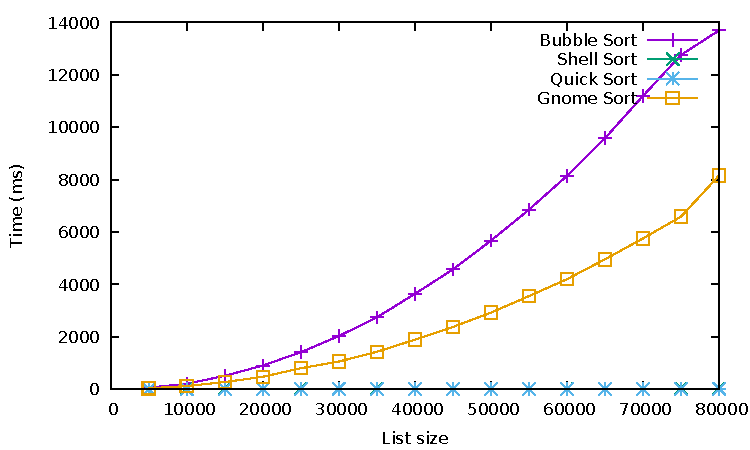
\includegraphics[page=1,width=\linewidth]{labpal-plots.pdf}}
\end{lrbox}



This is a simple \LaTeX{} document showing how to include plots, macros and
tables generated with LabPal inside your research paper. Our paper will use the
data generated by the \emph{Sorting Lab} example contained in LabPal's example
folder.

\section*{Required Packages}

Make sure your \LaTeX{} file imports the following packages:

\begin{itemize}
\item \texttt{graphicx} and \texttt{pdfpages} to include figures
\item \texttt{multirow} for tables
\item \texttt{hyperref} for the hyperlink functionalities
\end{itemize}

\section*{Importing the Files}

The first step is to run the experiments in the lab, and to export three files:

\begin{itemize}
\item The PDF files for all plots in the lab. Go to the \textsl{Plots} page and
click on the ``Download all plots'' button. By default, the file is called
\verb+labpal-plots.pdf+.
\item The macro file to easily import the plots. In the \textsl{Plots} page,
click on the ``Download \LaTeX{} macros'' button. By default, the file is called
\verb+labpal-plots.tex+.
\item The \LaTeX{} file for the tables. In the \textsl{Tables} page, click on
the ``Download all tables'' button. By default, the file is called
\verb+labpal-tables.tex+.
\end{itemize}

Copy these three files in the same folder as your research paper. At the top
of the paper, make sure you include the two \texttt{.tex} files using the \texttt{input}
command.

\section*{Adding a Table}

To add a table to your text, create a \texttt{table} environment as usual. Use
the command \verb+\usebox{\boxname}+ to include the contents of a table, where
\verb+boxname+ is the name of one of the boxes defined in
\verb+labpal-tables.tex+. (In your lab, you can set the name given to each
table's box through method \verb+setNickname()+. Otherwise, LabPal assigns a
default name to each table.)

\begin{table}
\centering
\usebox{\sorttime}
\caption{This table is generated by LabPal. Hyperlinks in the table refer to
individual data points in the lab.}
\label{table-sort}
\end{table}

Table \ref{table-sort} shows an example of a table included in such a way. Each
cell in the table is a hyperlink. The destination of each link can be
copy-pasted in LabPal's web console, in the \textsl{Find} page, which takes you
to the table, plot or macro where this specific data point is defined.

\section*{Adding a Plot}

Adding a plot can be done in the same way as a table; create a \texttt{figure}
environment, and use the \verb+\usebox{\boxname}+ to include a specific image;
\verb+boxname+ is the name of one of the boxes defined in
\verb+labpal-plots.tex+.

\begin{figure}
\centering
\usebox{\sortplot}
\caption{This plot is generated by LabPal. The hyperlink points to the same
figure inside the lab instance.}
\end{figure}

Figure \ref{table-sort} shows an example of a figure included in such a way. The
figure is surrounded by a hyperlink. The destination of this link can be
copy-pasted in LabPal's web console, in the \textsl{Find} page, which takes you
to the plot and its associated data table.

\end{document}